\chapter{PCB 2.0 设计和测试}
\label{cha:PCB-v2}

本章设计源文件和历史版本详见\url{https://github.com/TingliangZhang/Misaka-PCB-v2}

\section{需要解决的问题}

在测试版本的PCB(PCB v1)中出现了不少经过测试发现的问题,在第二版本中尽可能予以纠正:

\begin{itemize}
    \item ATmega2560的晶振封装无法手焊,而且不在嘉立创基础库里,不方便SMT
    \item PowerSTEP01过于昂贵,而且极难手动贴片。
\end{itemize}

\section{设计环境的更改}

PCB的设计依赖电子设计自动化(英语:Electronic design automation,缩写:EDA)软件。

当初绘制PCB v1时使用的时Altium Designer 20.0.9集成开发环境。

由于AD20是商业付费EDA软件,而且之前的绘制使用了Altium Live 在线供应商封装库,可移植性和便携性不是很好,即使生成了Integrated Library,也很难找到成套的规范化封装。另外AD20的源文件不是普通编辑器可以打开的文本,这使得Git代码管理变得困难。

基于以上考量,改用KiCAD开源EDA软件进行目前及将来的电路设计,如图~\ref{fig:kicad_flowchart}。

\begin{figure}[htbp]
    \centering
    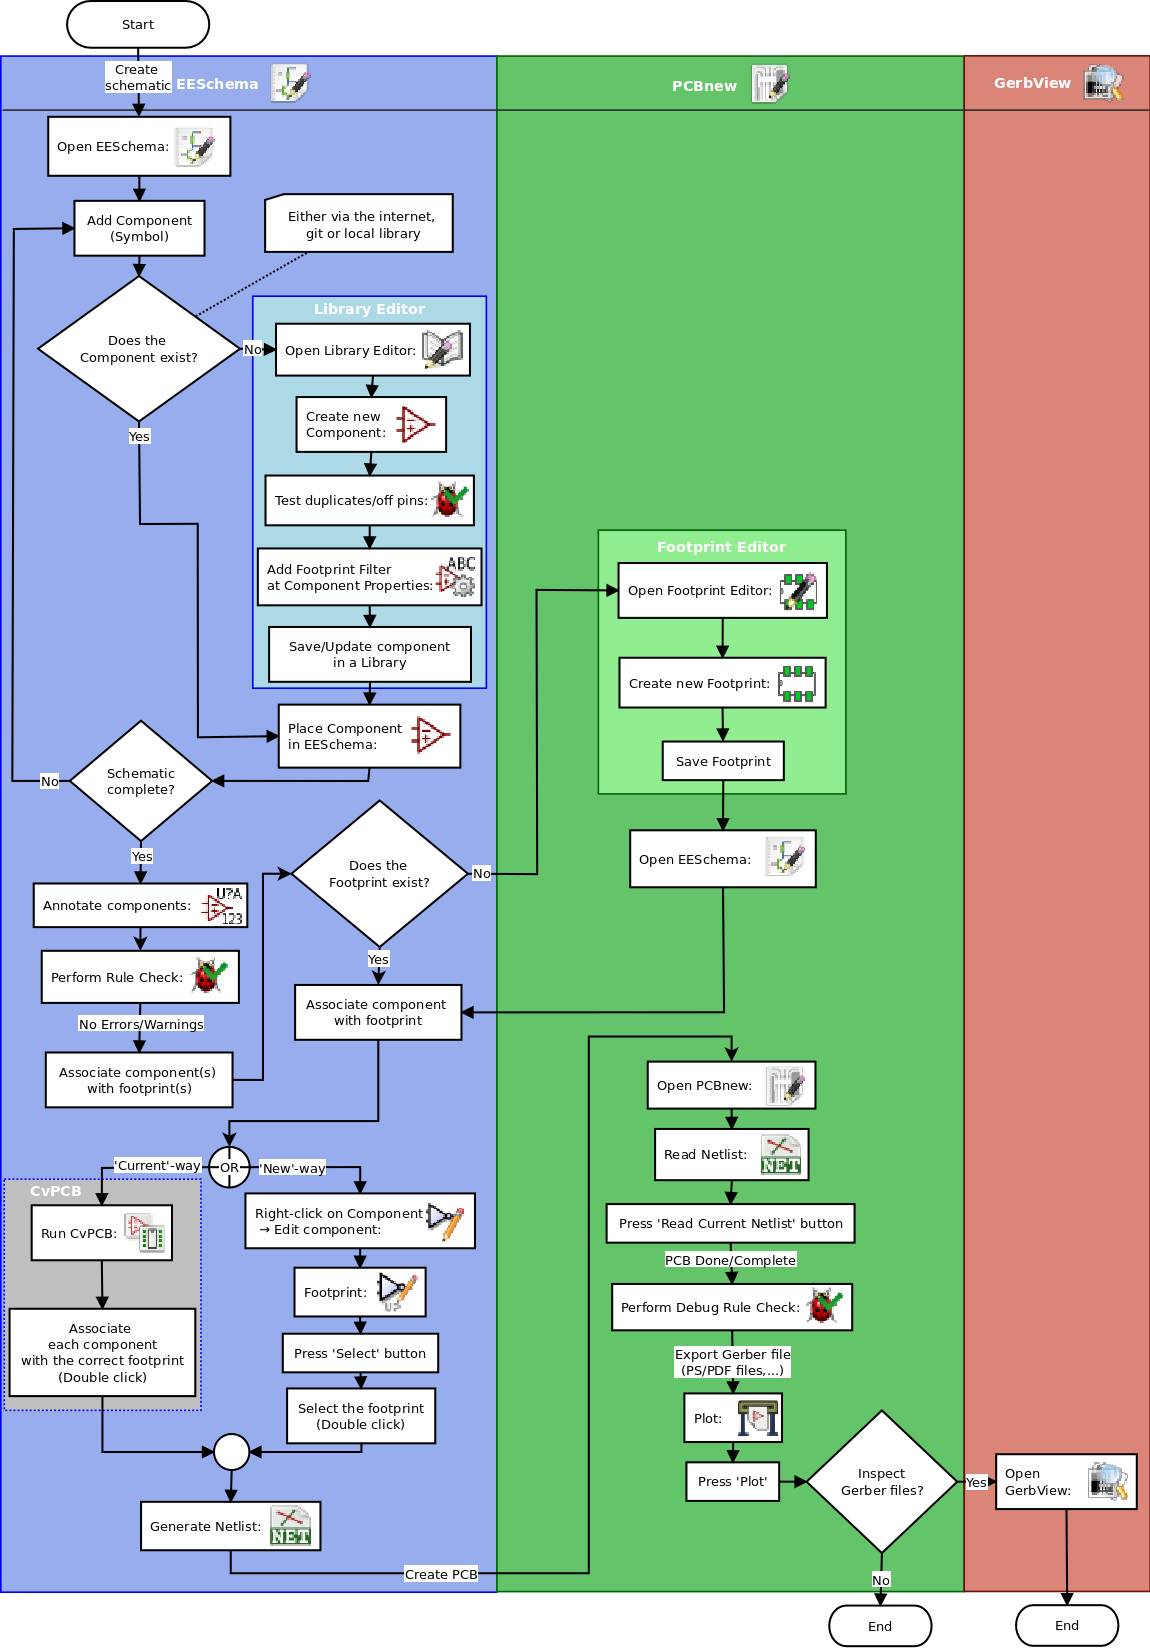
\includegraphics[width=\columnwidth]{kicad_flowchart.png}
    \caption{KiCad Workflow}
    \label{fig:kicad_flowchart}
\end{figure}

\section{MCU}

参考了Mega Pro Embed CH340G / ATmega2560 board \footnote{\url{https://robotdyn.com/mega-2560-pro-embed-ch340g-atmega2560-16au.html}}的设计,如图~\ref{fig:MEGA-PRO-CH340GATmega2560}。

\begin{figure}[htbp]
    \centering
    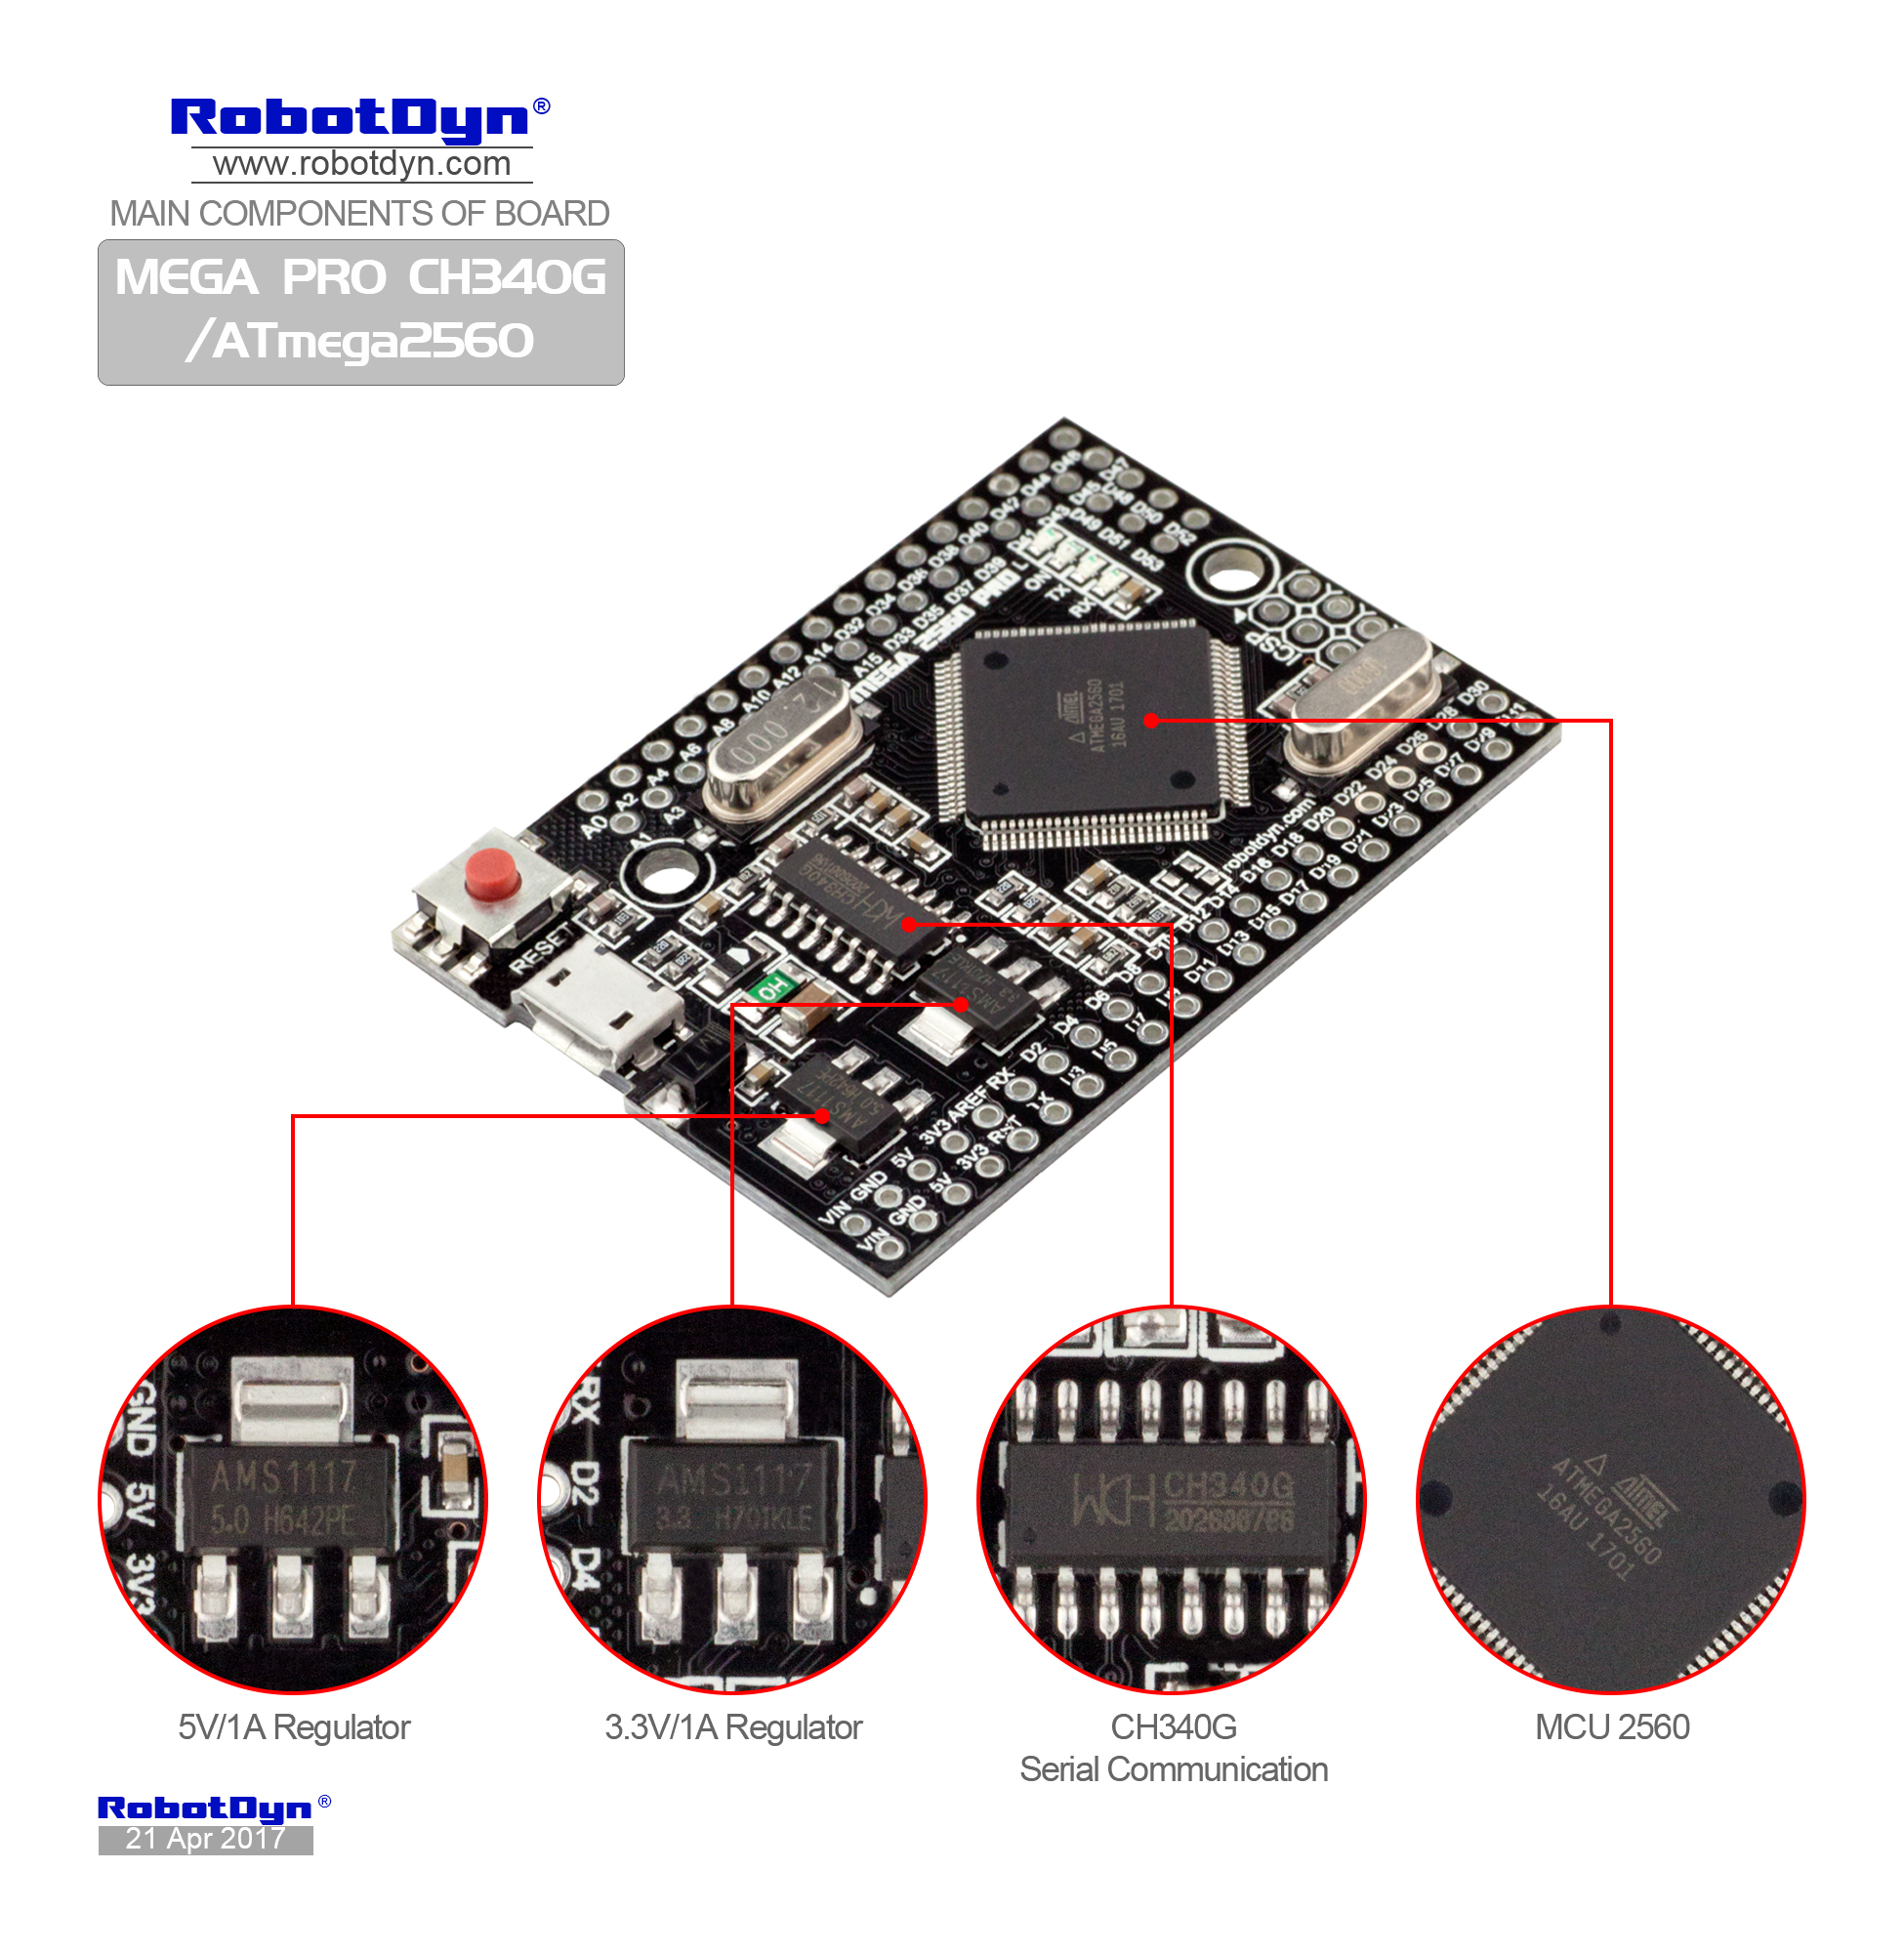
\includegraphics[width=\columnwidth]{MEGA-PRO-CH340GATmega2560.jpg}
    \caption{Mega Pro Embed CH340G / ATmega2560}
    \label{fig:MEGA-PRO-CH340GATmega2560}
\end{figure}


\section{晶振}

由于陶瓷谐振器大多需要外加电容,且封装很难拿手焊,所以选用陶瓷振荡子。

MURATA的 CSTLS16M0X51-A0 \footnote{\url{https://www.murata.com/zh-cn/products/productdetail?partno=CSTLS16M0X51-B0}}。

村田的CSTLS系列陶瓷振荡子(CERALOCK)特征如下:

\begin{enumerate}
    \item 无需外部负载电容器即可构建振荡电路。系列产品拥有内置电容值各不相同的各种型号,可适用于各种集成电路。
    \item 在宽温度范围内稳定。
    \item 结构小巧、重量轻并表现出优异的耐冲击性能。
    \item 可以设计用无需调校的振荡器电路
    \item 性价比高,可用性可靠。
\end{enumerate}



\section{USB UART 异步串行数据传输芯片}

USB转UART芯片稳定程度和价格均为FT232>CH340>PL2303。

FT232RL-REEL价格最贵,1片要27.61,1000+批量价格也要16.24每个。FT232RL/BL的优势就FTDI一直在更新驱动发布在官网,驱动经过微软认证,兼容性最好。内部固化了USB底层协议,转出来的是虚拟串口,可以固定COM口号。电路简单,数据传输稳定性好。FT232RL自带晶振,可以转RS232/TTL(常用)及RS422,RS485 高端市场专用。

PL2303最便宜,但波特率在115200时就有可能出现延迟。

经过测试,CH340\footnote{\url{http://www.wch.cn/products/CH340.html}}可以满足需求,且批量购买1000+只要1.47一片。

CH340C

下图是统一供电方式下MCU 单片机通过TTL 串口连接CH340 芯片实现USB通讯的参考电路。该产品选择自供电方式,VCC 支持5V 或者3.3V(VCC 为3.3V 时V3 需短接到VCC),完全不使用USB 总线电源VBUS(如有需要MCU可以通过I/O 串电阻后检测其是否有效)。CH340 与MCU 使用同一电源VCC,所以CH340与MCU 之间不存在双电源通过I/O相互电流倒灌的情形。

CH340没有使用到的信号线都可以悬空。对于CH340C/N/K/E/B 芯片,无需X6 和C17 及C18。

\section{供电}

考虑使用USB PD

USB PD等多快充协议芯片CH236\footnote{\url{http://www.wch.cn/products/CH236.html}}